% =====================================================================
%  Zusammenfassung IAUT -- Teil Automatisierung (HS26) -- LaTeX-Quelle
%  Kompilieren: pdflatex (2x) oder latexmk -pdf main.tex
%  In VS Code mit der Extension "LaTeX Workshop": main.tex öffnen,
%  speichern (Ctrl+S) baut automatisch, Ctrl+Alt+V zeigt das PDF.
%
%  Format: A4 hoch, 2 Spalten, 8pt.
%  Inhalt: eine Datei pro Block in sections/
% =====================================================================
\documentclass[8pt]{extarticle}

% ---------------------------------------------------------------------
% Pakete
% ---------------------------------------------------------------------
\usepackage[utf8]{inputenc}
\usepackage[T1]{fontenc}
\IfFileExists{ngerman.ldf}{\usepackage[ngerman]{babel}}{%
  \renewcommand{\contentsname}{Inhaltsverzeichnis}}
\usepackage{helvet}
\renewcommand{\familydefault}{\sfdefault}

\usepackage[a4paper,left=1.0cm,right=1.0cm,top=1.0cm,bottom=1.1cm,
            footskip=0.5cm]{geometry}
\usepackage{amsmath,amssymb}
\usepackage{graphicx}
\usepackage{multicol}
\usepackage{booktabs}
\usepackage{array}
\usepackage{tabularx}
\usepackage{environ}        % damit tabularx in \ztab funktioniert
\usepackage{enumitem}
\usepackage[dvipsnames]{xcolor}
\usepackage{titlesec}
\usepackage[most]{tcolorbox}
\usepackage{listings}
\usepackage{fancyhdr}
\usepackage{lastpage}
\usepackage{tikz}
\usetikzlibrary{automata,positioning,arrows.meta}
\usepackage[colorlinks=true,linkcolor=blue!60,urlcolor=blue!60]{hyperref}

\graphicspath{{figures/}}

% ---------------------------------------------------------------------
% Metadaten (hier anpassen)
% ---------------------------------------------------------------------
\newcommand{\doctitle}{Zusammenfassung - IAUT Automatisierung}
\newcommand{\docauthors}{Jan Vogel}
\newcommand{\docdate}{\today}
\newcommand{\docversion}{v1.0}

% ---------------------------------------------------------------------
% Layout: 2 Spalten, Abstände
% Platz knapp? Zuerst hier an den Rändern drehen, dann an der
% Schriftgrösse in \documentclass ganz oben.
% ---------------------------------------------------------------------
\setlength{\columnsep}{10pt}
\setlength{\columnseprule}{0.4pt}
\renewcommand{\columnseprulecolor}{\color{black!30}}
\setlength{\parindent}{0pt}
\setlength{\parskip}{0.5pt}
\setlength{\tabcolsep}{3pt}
\setcounter{secnumdepth}{2}
\setcounter{tocdepth}{1}

\setlist[itemize]{nosep,leftmargin=1.1em,topsep=1pt,label=\textcolor{blockacc}{\textbullet}}
\setlist[enumerate]{nosep,leftmargin=1.5em,topsep=1pt}
\setlist[description]{nosep,topsep=1pt,leftmargin=0pt,font=\normalfont\bfseries}

\setlength{\jot}{5pt}
\allowdisplaybreaks
\AtBeginDocument{%
  \setlength{\abovedisplayskip}{3pt}\setlength{\belowdisplayskip}{3pt}%
  \setlength{\abovedisplayshortskip}{3pt}\setlength{\belowdisplayshortskip}{3pt}}

% ---------------------------------------------------------------------
% Farben: eine pro Block
% Beim Durchblättern erkennt man den Block an der Balkenfarbe.
% ---------------------------------------------------------------------
\definecolor{cB1}{HTML}{1F4E79}   % Grundlagen Automatisierung
\definecolor{cB2}{HTML}{2E7D32}   % TwinCAT / SPS
\definecolor{cB3}{HTML}{B35C00}   % Strukturierter Text
\definecolor{cB4}{HTML}{6A1B9A}   % Signale & digitale Filter
\definecolor{cB5}{HTML}{B3261E}   % Zustandsautomaten
\definecolor{cB6}{HTML}{00695C}   % Tasks / EtherCAT
\definecolor{cB7}{HTML}{8D6E00}   % PID & Anti-Windup
\definecolor{cB8}{HTML}{AD1457}   % Safety
\definecolor{cREF}{HTML}{37474F}  % Referenzteil
\colorlet{blockacc}{cREF}         % Akzentfarbe des aktuellen Blocks
\colorlet{blockbar}{cREF!16}      % Balkenfarbe = helle Variante

% ---------------------------------------------------------------------
% Überschriften als farbige Balken
% ---------------------------------------------------------------------
\titleformat{\section}[block]{\normalfont}{}{0pt}{\sectionbar}
\titleformat{name=\section,numberless}[block]{\normalfont}{}{0pt}{\sectionbarnonum}
\titleformat{\subsection}[block]{\normalfont}{}{0pt}{\subsectionbar}
\newcommand{\sectionbar}[1]{\colorbox{blockbar}{\parbox{\dimexpr\linewidth-2\fboxsep\relax}{\large\strut\textcolor{blockacc}{\textbf{\thesection\ #1}}}}}
\newcommand{\sectionbarnonum}[1]{\colorbox{blockbar}{\parbox{\dimexpr\linewidth-2\fboxsep\relax}{\large\strut\textcolor{blockacc}{\textbf{#1}}}}}
\newcommand{\subsectionbar}[1]{{\color{blockacc}\rule{2pt}{8pt}}\hskip3pt{\footnotesize\textbf{\thesubsection\ #1}}}

\titlespacing*{\section}{0pt}{4pt}{1.5pt}
\titlespacing*{\subsection}{0pt}{4pt}{1pt}

% Blockueberschrift: setzt die Farbe und schreibt den Balken.
%   \vlsec{Farbe}{Kurzlabel}{Titel}
\newcommand{\vlsec}[3]{%
  \colorlet{blockacc}{#1}%
  \colorlet{blockbar}{#1!16}%
  \section[{#2 -- #3}]{#3\hfill\normalsize #2}%
}

% ---------------------------------------------------------------------
% Kopf-/Fusszeile
% ---------------------------------------------------------------------
\pagestyle{fancy}
\fancyhf{}
\renewcommand{\headrulewidth}{0pt}
\renewcommand{\footrulewidth}{0.4pt}
\fancyfoot[L]{\tiny \docauthors\ --- Zusammenfassung --- IAUT Automatisierung --- \docversion}
\fancyfoot[R]{\tiny \thepage/ \pageref{LastPage}}

% ---------------------------------------------------------------------
% Eigene Umgebungen und Befehle
% ---------------------------------------------------------------------
\newcommand{\R}[1]{\texttt{#1}}          % Variable / Code / Schluesselwort
\newcommand{\T}[1]{\textbf{#1}}          % Schluesselbegriff
\newcommand{\ra}{\,$\rightarrow$\,}
\newcommand{\SW}[1]{\textcolor{blockacc}{\textbf{#1}}\hskip0.4em}  % Stichwort am Zeilenanfang
\newcommand{\JA}{\textcolor{green!45!black}{\textbf{Ja}}}
\newcommand{\NEIN}{\textcolor{red!70!black}{\textbf{Nein}}}

% Kompakte Tabelle ueber die Spaltenbreite. Erste Zeile = Kopfzeile.
%   \begin{ztab}{@{}Xr@{}} Kopf & Kopf \\ \midrule ... \end{ztab}
% (\NewEnviron statt \newenvironment, sonst findet tabularx sein Ende nicht)
\NewEnviron{ztab}[1]{%
  \par\footnotesize
  \begin{tabularx}{\linewidth}{#1}\toprule\BODY\bottomrule\end{tabularx}%
  \par\vspace{1pt}\normalsize}

% Boxen
\tcbset{zfbox/.style={enhanced,arc=1.5mm,boxrule=0.6pt,
  left=3pt,right=3pt,top=2pt,bottom=2pt,
  fonttitle=\sffamily\bfseries\footnotesize,fontupper=\footnotesize,
  before skip=2.5pt,after skip=2.5pt}}

\newtcolorbox{formel}[1][]{zfbox,colback=blockacc!4,colframe=blockacc,
  coltitle=white,colbacktitle=blockacc,title={#1}}       % Formel/Kernaussage
\newtcolorbox{falle}[1][Falle]{zfbox,colback=red!4,colframe=red!65,
  coltitle=white,colbacktitle=red!65,title={#1}}         % typischer Fehler
\newtcolorbox{rezept}[1][Rezept]{zfbox,colback=green!4,colframe=green!40!black,
  coltitle=white,colbacktitle=green!40!black,title={#1}} % Schritt fuer Schritt
\newtcolorbox{bsp}[1][Beispiel]{zfbox,colback=yellow!8,colframe=black!55,
  coltitle=white,colbacktitle=black!55,title={#1}}       % durchgerechnet
\newtcolorbox{achtung}[1][Achtung]{zfbox,colback=red!4,colframe=red!65,
  coltitle=white,colbacktitle=red!65,title={#1}}

% Bild in Spaltenbreite (Anteil von \linewidth)
\newcommand{\fig}[2][0.9]{\par\vspace{2pt}{\centering\includegraphics[width=#1\linewidth]{#2}\par}\vspace{1pt}}

% Code: Strukturierter Text (IEC 61131-3)
\lstdefinelanguage{ST}{
  sensitive=true,
  morekeywords={PROGRAM,END_PROGRAM,FUNCTION,END_FUNCTION,FUNCTION_BLOCK,
    END_FUNCTION_BLOCK,VAR,VAR_INPUT,VAR_OUTPUT,VAR_IN_OUT,VAR_GLOBAL,
    CONSTANT,RETAIN,PERSISTENT,END_VAR,AT,TYPE,END_TYPE,STRUCT,END_STRUCT,
    IF,THEN,ELSIF,ELSE,END_IF,CASE,OF,END_CASE,FOR,TO,BY,DO,END_FOR,
    WHILE,END_WHILE,REPEAT,UNTIL,END_REPEAT,EXIT,RETURN,
    AND,OR,XOR,NOT,MOD,TRUE,FALSE,ARRAY},
  morekeywords=[2]{BOOL,BYTE,WORD,DWORD,LWORD,SINT,INT,DINT,LINT,USINT,
    UINT,UDINT,ULINT,REAL,LREAL,TIME,STRING},
  morekeywords=[3]{TON,TOF,TP,R_TRIG,F_TRIG,SHL,SHR,SQRT,SIN,EXPT,
    REAL_TO_INT,INT_TO_REAL,WORD_TO_INT},
  morecomment=[l]{//},
  morecomment=[s]{(*}{*)}
}
\lstset{
  language=ST,
  basicstyle=\ttfamily\scriptsize,
  keywordstyle=\color{blockacc}\bfseries,
  keywordstyle=[2]\color{black!70}\bfseries,
  keywordstyle=[3]\color{blockacc},
  columns=fullflexible, keepspaces=true,
  aboveskip=2pt, belowskip=2pt, xleftmargin=3pt,
  commentstyle=\color{black!55},
  literate={ä}{{\"a}}1 {ö}{{\"o}}1 {ü}{{\"u}}1 {Ä}{{\"A}}1 {Ö}{{\"O}}1
           {Ü}{{\"U}}1 {ß}{{\ss}}1
}

% =====================================================================
\begin{document}

% ------------------------- Kopf + Inhalt -----------------------------
% Kein \newpage nach dem Kopf: alles laeuft in einem Spaltenfluss.
\begin{multicols*}{2}
  {\centering
   {\Large\bfseries \doctitle\par}\vspace{1pt}
   {\footnotesize Skript v1.4, Aufgabenserien 1--9, Folien
    \quad\textbullet\quad \docauthors
    \quad\textbullet\quad \docdate\par}}
  \vspace{4pt}
  % !TEX root = ../main.tex
% ---------------------------------------------------------------------
%  Navigation: Farblegende + "Wenn die Aufgabe lautet ..."
%  Steht auf der Titelseite, vor dem Inhaltsverzeichnis.
% ---------------------------------------------------------------------

\begin{tcolorbox}[zfbox, colback=black!2, colframe=black!45,
  coltitle=white, colbacktitle=black!45, title={Farbcode der Blöcke}]
\textcolor{cB1}{\rule{7pt}{7pt}}~\T{B1} Grundlagen \quad
\textcolor{cB2}{\rule{7pt}{7pt}}~\T{B2} TwinCAT/SPS \quad
\textcolor{cB3}{\rule{7pt}{7pt}}~\T{B3} ST \quad
\textcolor{cB4}{\rule{7pt}{7pt}}~\T{B4} Filter \\
\textcolor{cB5}{\rule{7pt}{7pt}}~\T{B5} Automaten \quad
\textcolor{cB6}{\rule{7pt}{7pt}}~\T{B6} Tasks/EtherCAT \quad
\textcolor{cB7}{\rule{7pt}{7pt}}~\T{B7} PID \quad
\textcolor{cB8}{\rule{7pt}{7pt}}~\T{B8} Safety \\[3pt]
\textcolor{cREF}{\rule{7pt}{7pt}}\,Formel \;
\textcolor{red!65}{\rule{7pt}{7pt}}\,Falle \;
\textcolor{green!40!black}{\rule{7pt}{7pt}}\,Rezept \;
\textcolor{black!55}{\rule{7pt}{7pt}}\,Beispiel \\[3pt]
\T{MEP:} 120\,min, 120\,Punkte (1\,Punkt $\approx$ 1\,Minute), alle
Papierunterlagen erlaubt, Code \emph{auf Papier}. Ja/Nein-Fragen:
falsch $=-1$ \ra bei Unsicherheit leer lassen.
Abschnitt~11 ist ein Stichwortregister.
\end{tcolorbox}

\begin{tcolorbox}[zfbox, colback=black!2, colframe=black!45,
  coltitle=white, colbacktitle=black!45, title={Wenn die Aufgabe lautet \dots}]
\begin{tabularx}{\linewidth}{@{}Xr@{}}
Ja/Nein-Fragebogen (HS24, mit Begründung) & \ref{sec:quiz} \\
Variable in GVL mit Klemme verknüpfen & \ref{rez:gvlio} \\
Sensorspannung \ra physikalische Grösse & \ref{rez:skalierung} \\
Warum reicht eine \R{FUNCTION}? & \ref{sec:pou} \\
$G(s)$ mit $s=\frac{1-z^{-1}}{T}$ diskretisieren & \ref{rez:diskret} \\
Differenzengleichung als FB programmieren & \ref{bsp:fbfilter} \\
Zustandsdiagramm skizzieren, ENUM + CASE & \ref{rez:automat} \\
Förderband-Automat komplett (MEP HS24) & \ref{bsp:foerderband} \\
Ampel mit Timern, Hand/Automatik & \ref{bsp:ampel} \\
Zweite Anlage mit gleicher Logik & \ref{falle:instanz} \\
Timer (\R{TON}/\R{TOF}/\R{TP}) richtig einsetzen & \ref{sec:timer} \\
Flanke / Doppelklick erkennen & \ref{bsp:edge} \\
Statuswort zerlegen, \R{SHR}/\R{SHL}, Hex & \ref{rez:statuswort} \\
Gleitender Mittelwert / Forgetting Factor & \ref{sec:mittelwert} \\
PID diskretisieren (P, I-Trapez, D gefiltert) & \ref{rez:pid} \\
Anti-Reset-Windup (Back-Calculation) & \ref{sec:arw} \\
Tasks: Basiszeit, Priorität, Zeitverlauf & \ref{bsp:tasks} \\
EtherCAT: on-the-fly, in-place, WC & \ref{sec:ethercat} \\
RETAIN vs.\ PERSISTENT & \ref{sec:remanenz} \\
\end{tabularx}
\end{tcolorbox}

  \vspace{2pt}
  \tableofcontents
  \vspace{3pt}

  % !TEX root = ../main.tex
% ---------------------------------------------------------------------
%  B1 -- Grundlagen der Automatisierung (Skript Kap. 1, Folien)
% ---------------------------------------------------------------------
\vlsec{cB1}{B1}{Grundlagen der Automatisierung}
\label{sec:grundlagen}

\SW{Definition} (DIN 19222) Ausrüsten einer Einrichtung, so dass sie
\emph{ganz oder teilweise ohne Mitwirkung des Menschen} geschieht. Der
Mensch legt fest \emph{was} geschieht (Programm), nicht mehr \emph{wie}.

\SW{Vier Gebiete} \T{Maschinen}- (Presse, Roboter), \T{Anlagen}-
(Kraftwerk, Chemie, mehrere vernetzte Regelkreise), \T{Gebäude}- (Heizung,
Lüftung, Licht), \T{Geräte}automatisierung (Insulinpumpe, Saugroboter).
Modul-Fokus: Maschinen und Anlagen.

\subsection{Automatisierungspyramide}
\begin{ztab}{@{}llX@{}}
Ebene & System & Zeit \\ \midrule
Firma & ERP & Tage--Monate \\
Produktion & MES & Stunden--Schichten \\
Anlage & Prozessleitsystem, SCADA & s--min \\
System & SPS (Station, Achse) & Sekunden \\
Sensor/Aktor & Regelung (PID) & ms \\
\end{ztab}
Nach \emph{unten}: mehr Datenpunkte, schnellere Reaktion. Nach \emph{oben}:
höherer Aggregationsgrad (Tausende Sensorwerte \ra eine Kennzahl).

\begin{formel}[Steuern vs.\ Regeln]
\T{Steuerung} = offener Wirkungsablauf (Steuerkette): Eingang beeinflusst
Ausgang, \emph{keine Rückmeldung}, ob das Ziel erreicht wurde
(Ablaufsteuerung, Zustandsautomat).\\
\T{Regelung} = geschlossener Wirkungskreis: Istwert wird gemessen, mit
Sollwert verglichen, die Regelabweichung wirkt zurück (PID).
\end{formel}
\SW{Beispiel Abkantpresse} Stempel über 2 Hydraulikzylinder geregelt;
Biegehilfen: 3 Achsen $\times$ 3 Kaskadenregler (Strom, Geschwindigkeit,
Position) $=9$ PID. Dazu reine Steuerung: Bedienung, HMI, Rezepturen,
Produktionsdaten, Safety (Lichtvorhang, Zweihand).

\subsection{Aufbau eines Automatisierungssystems}
HMI (Mensch) \ra SPS \ra Feldbus \ra Antriebe, Aktoren, Sensoren.
\begin{ztab}{@{}lX@{}}
mit Echtzeit & Regler, Prozessabläufe \\
ohne Echtzeit & HMI, Produktionsplanung, Archivierung \\
\end{ztab}
\SW{Anforderungen} Echtzeitfähigkeit (BS, Speicher), E/A von
Prozesssignalen, Sicherheit/Zuverlässigkeit (Redundanz), Resistenz gegen
Umwelt (Gehäuse, Schaltschrank).

\SW{Bauformen} Control Panel (mit Bildschirm), Compact (Hutschiene, wie
CX im Labor), 19''-Rack-Industrie-PC.
\T{SPS}: Wenn-Dann-Logik + Zustandsspeicher. \T{CNC}: Bahnregelung,
CAD-Import (IGES/DXF). \T{Industrie-PC}: gehärteter PC + Soft-SPS
(TwinCAT) \ra SPS und HMI in einem.

\SW{Schaltschrank} Hauptschalter \ra Sicherungsautomaten \ra Netzteil
(230/400\,V AC \ra 24\,V DC) \ra SPS \ra E/A-Klemmen \ra
Frequenzumrichter (drehzahlvariable Antriebe) \ra Schütze/Relais (grosse
Lasten, trennen Steuer- von Leistungsebene) \ra Not-Aus-Kreis
(Sicherheitsrelais/Safety-SPS). Schutzart z.\,B.\ IP54.

\SW{I/O-Baum} \T{Online} (Scan der laufenden Hardware) oder \T{Offline}
(Klemmen aus Katalog, ESI-Dateien, nach Stückliste). EPLAN-Kopplung:
TF6360 importiert das Elektroschema.

\subsection{Feldbusse}
\label{sec:feldbus}
Gemeinsame Leitung statt Einzelverdrahtung (zentralisiert).
\begin{ztab}{@{}XX@{}}
Vorteile & Nachteile \\ \midrule
weniger Verkabelung & komplexer (Protokoll, Adressen) \\
einfach erweiterbar & teurer, Bus-Analyzer nötig \\
 & ev.\ längere Reaktionszeit \\
\end{ztab}
\SW{Generationen} klassisch: Profibus (RS-485), CAN/CANopen (Auto,
J1939). Ethernet-basiert: \T{EtherCAT} (Beckhoff), Profinet, EtherNet/IP,
SERCOS III. Gebäude: LON, EIB/KNX.

\begin{formel}[EtherCAT vs.\ TCP/IP]
\T{Gleiches Kabel} (Schicht 1, Cat5/RJ45, 100BASE-TX), aber
\emph{kein} IP und \emph{kein} TCP/UDP im Echtzeitpfad: eigener Ethertype
direkt auf Schicht 2, Verarbeitung on-the-fly, feste projektierte
Teilnehmer-Reihenfolge statt Routing, kein CSMA/CD \ra deterministisch,
$\mu$s bis wenige ms.
\end{formel}
\SW{Topologien} Linie (bis 100\,m zwischen Teilnehmern), Baum/Abzweig,
Stern (Junctions), \T{Ring mit Kabelredundanz} (letzter Teilnehmer zurück
zum Master: Kabelbruch \ra Gegenrichtung übernimmt). Fremdgeräte direkt
mit EtherCAT (Schunk-Greifer, Bota-Kraftsensor).

\subsection{Programmiersprachen IEC 61131-3}
\label{sec:sprachen}
\begin{ztab}{@{}llX@{}}
Sprache & Typ & Merkmal \\ \midrule
AWL / IL & textuell & SPS-Assembler, keine Schleifen, veraltet \\
KOP / LD & grafisch & Ersatz für Relaislogik, nicht für Komplexes \\
FBS / FBD & grafisch & Bit-Verknüpfungen, Datenfluss übersichtlich \\
\T{ST} & textuell & Hochsprache (Pascal/C), Schleifen, in Europa verbreitet \\
AS / SFC & grafisch & Zustandsabläufe, gut lesbar \\
\end{ztab}
\begin{falle}[Anzahl Sprachen]
Es sind \T{fünf} Sprachen \emph{insgesamt} -- ST plus \emph{vier} weitere.
IEC 61131-3 ist die einzige weltweit gültige Norm und
herstellerübergreifend (nicht nur Beckhoff).
\end{falle}
\SW{Warum ST} Filter, PID, Automaten brauchen Schleifen, Arrays, REAL,
Fallunterscheidungen. Reiner Text \ra Diff, Git, Code-Review.
\SW{Ausblick} \T{EN 61499}: objektorientierte Weiterentwicklung, verteilte
ereignisgesteuerte FBs über mehrere Steuerungen. \T{Codegenerierung}:
Simulink PLC Coder, TwinCAT-Simulink, B\&R Automation Studio --
validierter Regler ohne Abschreibfehler, aber weniger Kontrolle über den
Code. Direkter vs.\ indirekter Reglerentwurf siehe \ref{sec:pid}.

  % !TEX root = ../main.tex
% ---------------------------------------------------------------------
%  B2 -- SPS und TwinCAT (Skript Kap. 2, Anhang B, D, F; AS 1)
% ---------------------------------------------------------------------
\vlsec{cB2}{B2}{SPS und TwinCAT}
\label{sec:twincat}

\begin{formel}[Scan-Zyklus einer SPS]
\T{1.} Alle Eingänge ins \T{Prozessabbild der Eingänge} (PAE) lesen
\ra \T{2.} Programm auf diesem eingefrorenen Abbild abarbeiten
\ra \T{3.} \T{Prozessabbild der Ausgänge} (PAA) auf die Klemmen schreiben.
Wiederholt mit fester Zykluszeit. Eine Eingangsänderung \emph{während}
des Zyklus wird erst im nächsten Zyklus sichtbar.
\end{formel}

\SW{TwinCAT} Soft-SPS: Echtzeitkern \emph{unter} Windows. Engineering
(Visual Studio + TwinCAT XAE) auf dem Entwicklungsrechner (ER), Runtime auf
dem Zielsystem (Labor: CX5010/CX9020). TwinCAT ist \emph{Software}, kein
Feldbus -- der Feldbus heisst EtherCAT.

\SW{LEDs} PWR grün $=$ Strom. TC \T{grün} $=$ Run-Modus (Boot-Projekt
läuft), TC \T{blau} $=$ Config-Modus.
\SW{Modi} \T{Config} (mit \T{Freerun}: Klemmen ohne Programm testen,
Reiter \emph{Online}), \T{Run} (Programm läuft).

\subsection{Vom leeren Projekt zum laufenden Programm}
\begin{rezept}[Ablauf (AS 1)]
\begin{enumerate}
\item ER und SPS ins \T{gleiche Subnetz} (statische IP), \R{ping}.
\item TwinCAT-XAE-Projekt \ra Zielsystem wählen \ra suchen \ra
  \T{Route zufügen} (siehe ADS unten).
\item E/A \ra Gerät 1 (EtherCAT) \ra \T{Scan} / \emph{Nach Boxen suchen}.
\item SPS-Projekt hinzufügen (\R{MAIN} entsteht), Task-Zykluszeit setzen
  (z.\,B.\ 5 Zyklusticks $=$ 5\,ms).
\item GVL mit \R{AT \%I*} / \R{AT \%Q*}-Variablen, Code schreiben.
\item \T{Projektmappe erstellen} (kompilieren).
\item \emph{Instance} \ra PlcTask Inputs/Outputs \ra \T{Verknüpfung ändern}
  -- es werden nur typ- und grössengleiche Prozessdaten angeboten.
\item \T{Konfiguration aktivieren} (Zuordnungen), Run-Modus.
\item SPS \ra \T{Einloggen} (lädt Programm) \ra \T{Start}.
\end{enumerate}
Jede Codeänderung: neu erstellen und neu laden. Online kann man Werte
\T{schreiben} oder \T{forcieren} (testen ohne Hardware).
\end{rezept}

\subsection{E/A-Variablen und Verknüpfung}
\label{rez:gvlio}
\begin{lstlisting}
{attribute 'qualified_only'}  // Zugriff nur als GVL_IO.xxx
VAR_GLOBAL
  bTasterGelb   AT %I* : BOOL;  // Eingang (EL1004)
  bLampeRot     AT %Q* : BOOL;  // Ausgang (EL2004)
  iSensorRoh    AT %I* : INT;   // Analog-Eingang (EL3004)
  iAnalogOut    AT %Q* : INT;   // Analog-Ausgang (EL4034/EL3034)
END_VAR
VAR_GLOBAL CONSTANT
  rT : REAL := 0.01;            // Abtastzeit (s)
END_VAR
\end{lstlisting}
\begin{formel}[AT-Adressen]
\R{\%I*} $=$ Eingang, \R{\%Q*} $=$ Ausgang, \R{*} $=$ Adresse vergibt
TwinCAT. Die Zuordnung zur Klemme passiert im Engineering, nicht im Code
\ra gleiche Software auf anderer Hardware. Typ muss passen: 16-Bit-Analog
\ra \R{INT}, Digital \ra \R{BOOL}. Ohne \R{AT} erscheint die Variable
\emph{nicht} im Prozessabbild.
\end{formel}
\begin{falle}[GVL ist nicht nur für Klemmen]
Globale Variablenlisten enthalten auch Konstanten
(\R{VAR\_GLOBAL CONSTANT}) und normale globale Daten. Mit
\R{qualified\_only} muss man \R{GVL\_IO.} immer davor schreiben.
\end{falle}

\SW{Analoge Klemmen} 0--10\,V $\leftrightarrow$ \R{INT} 0--32767.
10\,V am Ausgang \ra Wert 32767 ($=2^{15}-1$, grösster INT).
EL3004: 4 Kanäle, 12 Bit Auflösung, Rohwert ändert sich in 16er-Schritten.

\subsection{Projektstruktur (TwinCAT XAE)}
\begin{ztab}{@{}lX@{}}
SYSTEM & Tasks, Echtzeit, Lizenzen, Routen \\
MOTION & NC-Achsen (nicht im Labor) \\
SPS & IEC-61131-Projekte \\
SAFETY & TwinSAFE-Logik (eigene Logic-Klemme) \\
E/A & EtherCAT-Klemmen, Prozessabbild \\ \midrule
References & Bibliotheken (\R{Tc2\_Standard}: \R{TON}, \R{R\_TRIG}) \\
DUTs & eigene Typen: STRUCT, ENUM \\
GVLs / POUs & globale Variablen / Programmcode \\
VISUs & Visualisierung (+ VISU\_TASK, eigener langsamer Task) \\
.tmc & Symbolbeschreibung für ADS-Zugriff von aussen \\
Instance & mit Hardware verknüpfte Instanz (PlcTask In/Out) \\
\end{ztab}

\SW{ADS} Beckhoff-Protokoll über TCP/IP für Download, Start/Stopp,
Online-Monitoring. Ziel $=$ (\T{AMS Net Id}, ADS-Port); AMS Net Id
z.\,B.\ \R{5.62.71.101.1.1} (oft IP + \R{.1.1}), bleibt bei IP-Wechsel.
\T{Route} $=$ Vertrauensbeziehung, sonst nimmt die SPS keine ADS-Befehle an.
Der \T{TwinCAT-Systemdienst} läuft immer (AMS-Router), auch ohne Visual
Studio.

\SW{CoE} Objektverzeichnis der Klemme (Index:Subindex, z.\,B.\
\R{0x8000:02}). EL3004 \R{0x80n0}: \R{:02} Presentation (\T{Signed} $=$
Zweierkomplement $=$ INT, darum direkt \R{INT\_TO\_REAL}), \R{:06}/\R{:15}
Filter, \R{:07} Grenzwert \ra Statusbit (die Klemme erkennt das
\emph{selbst}, ohne SPS). CoE-Online wirkt sofort, aber nur bis Neustart;
dauerhaft \ra \T{CoE-Startup}-Liste.

\subsection{Remanente Variablen}
\label{sec:remanenz}
\begin{ztab}{@{}lccc@{}}
Ereignis & normal & \R{RETAIN} & \R{PERSISTENT} \\ \midrule
Online Change & bleibt & bleibt & bleibt \\
Reset warm & weg & bleibt & bleibt \\
Reset kalt & weg & weg & bleibt \\
Neuer Download & weg & weg & bleibt \\
Reset Ursprung & weg & weg & weg \\
\end{ztab}
\begin{lstlisting}
VAR RETAIN     rIntegrator  : REAL; END_VAR
VAR PERSISTENT diStueckzahl : DINT; END_VAR
\end{lstlisting}
\SW{Wann was} Stückzähler über Programm-Update \ra \R{PERSISTENT}.
I-Anteil eines Reglers über kurzen Neustart \ra \R{RETAIN}.
\T{USV/UPS}: Akku/Kondensator überbrückt Stromausfall, Zeit zum Sichern.
\T{NOVRAM}: nichtflüchtiger RAM, jeden Zyklus beschreibbar.

  % !TEX root = ../main.tex
% ---------------------------------------------------------------------
%  B3 -- Strukturierter Text (Skript Kap. 3, Anhang C, E; AS 2)
% ---------------------------------------------------------------------
\vlsec{cB3}{B3}{Strukturierter Text (ST)}
\label{sec:st}

\subsection{POU-Typen: Funktion, Funktionsblock, Programm}
\label{sec:pou}
\begin{ztab}{@{}lXXX@{}}
 & \R{FUNCTION} & \R{FUNCTION\_BLOCK} & \R{PROGRAM} \\ \midrule
Gedächtnis & \T{nein} & ja (pro Instanz) & ja \\
Instanz & keine & \T{muss} instanziiert werden & genau eine, global \\
Rückgabe & 1 Wert über Namen (+ \R{VAR\_OUTPUT}) & beliebig viele \R{VAR\_OUTPUT} & Variablen \\
Aufruf & \R{x := F(a,b);} & \R{fb(in:=a); y:=fb.out;} & \R{P(); P.var} \\
Typisch & Umrechnung, Formel & Zähler, Filter, Flanke, Regler, Automat & \R{MAIN}, an Task \\
\end{ztab}
\begin{formel}[Wann reicht eine FUNCTION? (MEP-Frage)]
Wenn das Ergebnis \emph{nur vom aktuellen Eingang} abhängt -- z.\,B.\
Sensor-Rohwert \ra bar. Keine Werte aus früheren Zyklen nötig \ra kein
Gedächtnis \ra Funktion genügt. Sobald $y(k-1)$, $u(k-1)$, ein Timer oder
ein Zustand gebraucht wird \ra \R{FUNCTION\_BLOCK}.
\end{formel}
\SW{Programm-Variablen} von aussen lesbar mit \R{DoSomeMath.rSumme}.
Debugger: Breakpoint F9, Schritt F10/F8. Eine Funktion zeigt bei jedem
Aufruf frisch initialisierte lokale Variablen.

\subsection{Deklaration}
\begin{lstlisting}
FUNCTION F_Name : REAL        // Name : Rückgabetyp
VAR_INPUT  a, b : REAL;   END_VAR   // Kopie hinein
VAR_OUTPUT err  : BOOL;   END_VAR   // zusätzliche Ausgänge
VAR_IN_OUT arr  : ARRAY[*] OF INT; END_VAR // Referenz
VAR        tmp  : REAL := 0.0; END_VAR   // lokal
F_Name := a + b;              // Rückgabe = Funktionsname
\end{lstlisting}
Form immer \R{Name : Typ := Startwert;}. Ohne Startwert: 0 / \R{FALSE} /
0.0. Kommentare \R{(* *)} oder \R{//}. Zuweisung \R{:=}, Vergleich \R{=},
ungleich \R{<>}.

\subsection{Datentypen und Zahlendarstellung}
\begin{ztab}{@{}llX@{}}
Typ & Bit & Bereich / Zweck \\ \midrule
\R{BOOL} & 1 & TRUE/FALSE \\
\R{SINT}/\R{USINT} & 8 & $-128..127$ / $0..255$ \\
\R{INT}/\R{UINT} & 16 & $-32768..32767$ / $0..65535$ \\
\R{DINT}/\R{UDINT} & 32 & $\pm2.1\cdot10^9$ / $0..4.3\cdot10^9$ \\
\R{REAL}/\R{LREAL} & 32/64 & IEEE 754, $\approx$7 / 15 Stellen \\
\R{BYTE}..\R{LWORD} & 8..64 & Bitmuster, nur Bitoperationen \\
\R{TIME} & 32 & \R{T\#5S}, \R{T\#500MS}, \R{T\#1M30S} \\
\end{ztab}
\SW{Literale} \R{181} $=$ \R{2\#1011\_0101} $=$ \R{16\#B5}. Eine
Hex-Ziffer $=$ 4 Bit.
\SW{Zweierkomplement} negativ: alle Bits invertieren, $+1$.
$-5$ als INT $=$ \R{16\#FFFB}; dasselbe Bitmuster als UINT $=65531$.
Ein negativer Wert mehr als positive (INT bis $-32768$).
\SW{REAL} $(-1)^S\cdot1.M\cdot2^{E-127}$; $6.5=$ \R{16\#40D00000}.
0.1 ist nicht exakt darstellbar \ra REAL nie mit \R{=} vergleichen,
sondern mit Toleranz.

\subsection{Operatoren und Kontrollstrukturen}
Priorität: Klammern, Funktionsaufruf, \R{NOT}, \R{* / MOD}, \R{+ -},
Vergleiche, \R{AND}, \R{XOR}, \R{OR}. Im Zweifel klammern.
\begin{lstlisting}
IF a THEN ... ELSIF b THEN ... ELSE ... END_IF
CASE state OF
  ST_A:        ...;
  ST_B, ST_C:  ...;       // mehrere Werte
  1..3:        ...;       // Bereich
ELSE ...;
END_CASE
FOR i := 0 TO 9 BY 1 DO ... END_FOR    // feste Anzahl
WHILE bed DO ... END_WHILE            // prüft VOR Durchlauf
REPEAT ... UNTIL bed END_REPEAT       // prüft NACH: min. 1x
EXIT;     // innerste Schleife verlassen
RETURN;   // Baustein verlassen
\end{lstlisting}
\begin{falle}[WHILE in einer SPS]
Die ganze Schleife läuft in \emph{einem} Zyklus. Eingänge ändern sich
währenddessen nie (PAE ist eingefroren) \ra hängt die Abbruchbedingung an
einem Eingang, entsteht eine Endlosschleife \ra Zykluszeit-Überschreitung,
Task blockiert. Der SPS-Zyklus \emph{ist} schon die Schleife \ra lieber
\R{FOR} mit fester Anzahl oder pro Zyklus einen Schritt.
\end{falle}

\subsection{Arrays, Strukturen, Aufzählungen}
\begin{lstlisting}
arBuf : ARRAY[0..99] OF REAL;          // Index ausserhalb = Laufzeitfehler
arM   : ARRAY[0..3, 0..3] OF INT;      // 2D
arInit: ARRAY[0..4] OF REAL := [1.0, 2.5, 3.0, 0.5, 4.0];

TYPE ST_Status :                       // unter DUTs anlegen
STRUCT
  bTaster : BOOL;
  rVolt   : REAL;
END_STRUCT
END_TYPE
arHist : ARRAY[0..99] OF ST_Status;    // Array aus Strukturen
arHist[k].rVolt := 2.5;                // Punktnotation

TYPE E_Monat : (JANUAR := 1, FEBRUAR, MAERZ); END_TYPE
eM : E_Monat := JANUAR;
\end{lstlisting}
\begin{falle}[ENUM beginnt nicht \emph{immer} bei 0]
Ohne Angabe zählt TwinCAT ab 0 aufwärts -- man darf aber Werte setzen
(\R{JANUAR := 1}). Ein ENUM ist nur Lesbarkeit, im Maschinencode steht
eine Zahl.
\end{falle}
\SW{Array zurückgeben} Rückgabetyp \R{ARRAY[0..99] OF REAL} geht (feste
Grösse). Variable Länge nur als \R{VAR\_IN\_OUT arr : ARRAY[*] OF INT;}
mit \R{LOWER\_BOUND(arr,1)} / \R{UPPER\_BOUND(arr,1)} (liefern DINT).

\subsection{Typkonvertierung}
Keine impliziten Umwandlungen: immer \R{QUELLE\_TO\_ZIEL(x)}.
\R{REAL\_TO\_INT} rundet kaufmännisch, \R{TRUNC} schneidet ab,
\R{INT\_TO\_REAL} verlustfrei, \R{WORD\_TO\_INT}/\R{BOOL\_TO\_INT} für
Bitmuster.
\begin{falle}[Ganzzahldivision]
\R{INT / INT} bleibt INT: \R{7/2 = 3}. Für Skalierungen zuerst
\R{INT\_TO\_REAL} und mit \R{10.0} statt \R{10} rechnen.
\end{falle}

\subsection{Bitoperationen und Statuswort}
\label{rez:statuswort}
\R{SHR(x,n)} $=$ $x/2^n$ (rechts schieben), \R{SHL(x,n)} $=$ $x\cdot2^n$.
Einzelbit direkt: \R{w.6}. Setzen mit \R{OR}, löschen mit \R{AND NOT},
toggeln mit \R{XOR}.
\begin{rezept}[Bitfeld aus einem WORD extrahieren]
Maske mit \R{AND} \ra mit \R{SHR} an Stelle 0 schieben \ra konvertieren:
\R{inLength := WORD\_TO\_INT(SHR(sw AND 16\#FF00, 8));}\\
Einzelbit: \R{bOverrun := sw.6;} oder
\R{(SHR(sw,6) AND 16\#0001) = 1}.
\end{rezept}
\begin{bsp}[AS 2: Shift und Statuswort]
\R{myWord := 16\#5D7A} (23930). \R{SHR(myWord,3)} $=$ \R{16\#0BAF} $=$
2991 (Rest .25 fällt weg).\\
\R{SHL(WORD\_TO\_DWORD(myWord),3)} $=$ \R{16\#0002EBD0} $=$ 191440. Ohne
DWORD-Wandlung fallen die oberen Bits raus (\R{16\#EBD0}).\\
\R{myDWord OR 16\#F0000000} $=$ \R{16\#F002EBD0} (oberste 4 Bit gesetzt).\\[2pt]
RS232-Statuswort:\\
{\scriptsize\begin{tabular}{@{}l*{8}{c}@{}}
Bit & 15..8 & 7 & 6 & 5 & 4 & 3 & 2 & 1/0 \\
 & InLength & -- & OR & FR & PA & BUF\_F & IA & RR/TA \\
\end{tabular}}\\[2pt]
\begin{tabularx}{\linewidth}{@{}lrX@{}}
\R{16\#1D06} & 29 & IA, RR \\
\R{16\#534C} & 83 & OR\_ERR, BUF\_F, IA \\
\R{16\#C705} & 199 & IA, TA \\
\end{tabularx}
\end{bsp}

\subsection{Standardbausteine: Timer und Flanken}
\label{sec:timer}
\begin{ztab}{@{}lX@{}}
FB & Verhalten (Eingang \R{IN}, Zeit \R{PT}, Ausgang \R{Q}, \R{ET}) \\ \midrule
\R{TON} & Einschaltverzögert: \R{Q} wird TRUE, wenn \R{IN} schon \R{PT} lang TRUE ist. \R{IN}=FALSE \ra Reset. \\
\R{TOF} & Ausschaltverzögert: \R{Q} folgt \R{IN} sofort auf TRUE, bleibt nach Abfall noch \R{PT} TRUE. \\
\R{TP} & Puls: steigende Flanke \ra \R{Q} genau \R{PT} lang TRUE, nicht retriggerbar. \\
\R{R\_TRIG}/\R{F\_TRIG} & \R{CLK} \ra \R{Q} einen Zyklus TRUE bei steigender/fallender Flanke. \\
\R{CTU}/\R{CTD}, \R{RS}/\R{SR} & Zähler, Flipflops (gleiches Muster) \\
\end{ztab}
\begin{lstlisting}
VAR tonBlink : TON; bLampe : BOOL; END_VAR
// selbstrücksetzender Takt: toggelt alle 167 ms (= 3 Hz)
tonBlink(IN := bAktiv AND NOT tonBlink.Q, PT := T#167MS);
IF tonBlink.Q THEN bLampe := NOT bLampe; END_IF
\end{lstlisting}
\begin{falle}[Timer-Fallen]
Den Timer \T{jeden Zyklus} aufrufen (nicht nur im IF) -- sonst läuft
\R{ET} nicht. Zum Neustarten muss \R{IN} einen Zyklus FALSE sein. Im
Automaten \R{IN := (state = ST\_X)} schreiben, dann startet er beim
Zustandseintritt und setzt sich beim Verlassen selbst zurück.
Blinkfrequenz $f$: halbe Periode $=\frac{1}{2f}$.
\end{falle}

\begin{bsp}[EdgeDetector mit Doppelklick (AS 2)]
\label{bsp:edge}
\begin{lstlisting}
FUNCTION_BLOCK EdgeDetector
VAR_INPUT  inputValue : BOOL; tDouble : TIME := T#400MS; END_VAR
VAR_OUTPUT risingEdge, fallingEdge, doubleClick : BOOL; END_VAR
VAR        lastValue : BOOL; tpWin : TP; END_VAR

risingEdge  := inputValue AND NOT lastValue;
fallingEdge := NOT inputValue AND lastValue;
lastValue   := inputValue;          // Wert für nächsten Zyklus
doubleClick := risingEdge AND tpWin.Q;  // 2. Flanke im Fenster
tpWin(IN := risingEdge AND NOT doubleClick, PT := tDouble);
\end{lstlisting}
Eine Instanz pro Taster (\R{edgeGelb}, \R{edgeBlau}) -- jede hat ihr
eigenes \R{lastValue}.
\end{bsp}

  % !TEX root = ../main.tex
% ---------------------------------------------------------------------
%  B4 -- Signale, Sensoren, digitale Filter (Skript Kap. 3/4/6, Anh. A;
%        AS 2/3/5; Skript Digitale Regelung Kap. 2/3)
% ---------------------------------------------------------------------
\vlsec{cB4}{B4}{Signale, Sensoren, digitale Filter}
\label{sec:filter}

\subsection{Sensorwert umrechnen}
\label{rez:skalierung}
\begin{rezept}[Rohwert \ra Spannung \ra physikalische Grösse]
\T{1. Klemme:} $U=\dfrac{\text{INT}}{32767}\cdot10\,\text{V}$
\quad(EL3004: 0\,V $\leftrightarrow$ 0, 10\,V $\leftrightarrow$ 32767).\\
\T{2. Sensor linear} durch zwei Punkte $(U_1,p_1)$, $(U_2,p_2)$:
\[ p = p_1 + (U-U_1)\,\frac{p_2-p_1}{U_2-U_1} \]
\T{3. Ausgabe} zurück: $\text{INT}=\text{REAL\_TO\_INT}(U/10\cdot32767)$.
\end{rezept}
\begin{bsp}[MEP HS24: Drucksensor 1\,V $=$ 2\,bar, 10\,V $=$ 10\,bar]
Steigung $\frac{10-2}{10-1}=\frac{8}{9}$\,bar/V \ra
$p=2+(U-1)\cdot\frac{8}{9}$. Kontrolle: $U=5.5$\,V \ra $p=6$\,bar.
\begin{lstlisting}
FUNCTION F_SensorUmwandlung : REAL     // Rückgabe in bar
VAR_INPUT iRoh : INT; END_VAR
VAR       rU   : REAL; END_VAR
rU := INT_TO_REAL(iRoh) * 10.0 / 32767.0;      // V
F_SensorUmwandlung := 2.0 + (rU - 1.0) * 8.0 / 9.0;
\end{lstlisting}
Rückgabetyp \R{REAL} (Druck ist keine ganze Zahl). FUNCTION reicht,
weil kein Gedächtnis nötig ist (\ref{sec:pou}).
\end{bsp}
\SW{Ultraschall UB120-12GM} an EL3004, \T{single-ended} $=$ Spannung gegen
gemeinsame Masse (nicht differentiell). Soll die Anzeige im Ruhezustand
0\,V zeigen, obwohl der Sensor ohne Objekt Maximalspannung liefert:
$U_{\text{out}}=10-U$.

\subsection{Testsignale (AS 3)}
\label{sec:signale}
Zeit im Aufrufer hochzählen: \R{t := t + T;} ($T$ $=$ Zykluszeit in s).
\begin{lstlisting}
y := A * SIN(w * t) + yOff;               // Sinus
IF SIN(w * t) > 0.0 THEN y := yMax;       // Rechteck aus Sinus
ELSE y := yMin; END_IF
\end{lstlisting}
\begin{formel}[PWM als Funktionsblock (Zähler)]
Periode $T_0=\frac{2\pi}{\omega}$ muss ein \emph{ganzes} Vielfaches der
Zykluszeit sein: $N_2=T_0/T$ Zyklen pro Periode, $N_1=\text{Duty}\cdot N_2$
Zyklen \T{ein}. Zähler $<N_1$ \ra $y_{\max}$, sonst $y_{\min}$; bei $N_2$
auf 0. Auflösung $=N_2$ Stufen (z.\,B.\ $T=10$\,ms, $T_0=100$\,ms \ra nur
10 Duty-Werte, $f_0=10$\,Hz).
\end{formel}
\SW{TwinCAT Scope} misst Variablen \emph{direkt in der SPS} (YT-Chart,
Trace), kein physischer Messpunkt nötig. Projekt: \emph{TwinCAT
Measurement} \ra Scope YT \ra Target Browser \ra Record.

\subsection{Gleitender Mittelwert und Forgetting Factor}
\label{sec:mittelwert}
\begin{formel}[Mittelwert: nicht-rekursiv \ra rekursiv (exakt)]
\[M(k)=\frac1N\sum_{j=k-N}^{k}y(j)
\;\Rightarrow\; M(k)=M(k-1)+\frac1N\big(y(k)-y(k-N-1)\big)\]
Keine Näherung, nur weniger Rechnung (1 Add.\ + 1 Sub.\ statt $N$).
Ringpuffer bleibt nötig, weil $y(k-N-1)$ gebraucht wird.
\end{formel}
\begin{lstlisting}
FOR i := 0 TO 98 DO                    // Puffer nach links schieben
  arBuf[i] := arBuf[i + 1];
END_FOR
arBuf[99] := rNeu;                     // neuester Wert hinten
rSum := 0.0;
FOR i := 0 TO 99 DO rSum := rSum + arBuf[i]; END_FOR
rMittel := rSum / 100.0;
\end{lstlisting}
\begin{formel}[Forgetting Factor $\lambda<1$, $N\to\infty$]
Gewichteter Mittelwert, Nenner $1+\lambda+\lambda^2+\dots=\frac{1}{1-\lambda}$:
\[M(k)=(1-\lambda)\sum_{i\ge0}\lambda^i y(k-i)
=\lambda\,M(k-1)+(1-\lambda)\,y(k)\]
(Aufgabe schreibt $y(k-1)$: nur um einen Schritt verschobener Index.)
Kein Puffer, ein FB mit Gedächtnis \R{meanValue}. $\lambda\to1$: stärker
geglättet, träger; Faustregel $\approx\frac{1}{1-\lambda}$ Werte
($\lambda=0.95$ \ra 20).
\end{formel}
\begin{lstlisting}
meanValue := lambda * meanValue + (1.0 - lambda) * inputValue;
\end{lstlisting}

\subsection{Diskretisierung: von $G(s)$ zur Differenzengleichung}
\label{rez:diskret}
\begin{ztab}{@{}lll@{}}
Methode & Ersetzung & Eigenschaft \\ \midrule
Euler vorwärts & $s\approx\frac{z-1}{T}$ & einfach, kann instabil werden \\
\T{Euler rückwärts} & $s\approx\frac{1-z^{-1}}{T}$ & stabil bleibt stabil \\
Tustin / Trapez & $s\approx\frac2T\frac{1-z^{-1}}{1+z^{-1}}$ & am genausten \\
\end{ztab}
\begin{rezept}[Diskretisieren in 5 Schritten]
\begin{enumerate}
\item $s=\frac{1-z^{-1}}{T}$ in $G(s)$ einsetzen.
\item Doppelbruch auflösen: Zähler \emph{und} Nenner mit $T$ bzw.\ $T^2$
  multiplizieren.
\item Nenner nach Potenzen $z^0,z^{-1},z^{-2}$ ordnen.
\item Durch den $z^0$-Koeffizienten teilen \ra Nenner beginnt mit 1.
\item $z^{-i}\cdot Y\to y(k-i)$ (Verschiebungssatz), nach $y(k)$ auflösen.
\end{enumerate}
\T{Kontrolle:} DC-Verstärkung $H(z{=}1)=\frac{\sum b}{1+\sum a}$ muss gleich
$G(0)$ sein. Rekursiv (IIR) $=$ alte $y$ auf der rechten Seite;
nicht-rekursiv (FIR) $=$ nur $u$.
\end{rezept}

\begin{bsp}[Integrator, PT1, PT2 (Euler rückwärts)]
\T{Integrator} $\frac1s$: $y(k)=y(k-1)+T\,u(k)$ (vorwärts: $T\,u(k-1)$).\\[2pt]
\T{PT1} $\frac{1}{1+\tau s}$ \ra $\dfrac{T}{T+\tau-\tau z^{-1}}$:
\[y(k)=\frac{\tau}{\tau+T}\,y(k-1)+\frac{T}{\tau+T}\,u(k)\]
\T{PT2} $\frac{\omega_0^2}{s^2+2d\omega_0s+\omega_0^2}$, mit
$a_0=1+2d\omega_0T+\omega_0^2T^2$:
\[y(k)=\frac{(2+2d\omega_0T)\,y(k-1)-y(k-2)+\omega_0^2T^2\,u(k)}{a_0}\]
Eckfrequenz PT1 $\omega_e=1/\tau$; Resonanz PT2
$\omega_r=\omega_0\sqrt{1-2d^2}$.
\end{bsp}

\begin{bsp}[MEP HS24: Butterworth 2.\ Ordnung]
\label{bsp:fbfilter}
$G(s)=\dfrac{\omega_c^2}{s^2+\sqrt2\,\omega_cs+\omega_c^2}$,
$s^2=\frac{(1-z^{-1})^2}{T^2}=\frac{1-2z^{-1}+z^{-2}}{T^2}$.
Mal $T^2$:
\[H(z)=\frac{\omega_c^2T^2}{(1+\sqrt2\omega_cT+\omega_c^2T^2)
-(2+\sqrt2\omega_cT)z^{-1}+z^{-2}}\]
Mit $c=1+\sqrt2\,\omega_cT+\omega_c^2T^2$:
\[a_1=-\frac{2+\sqrt2\,\omega_cT}{c},\;
a_2=\frac1c,\;b_0=\frac{\omega_c^2T^2}{c},\;b_1=b_2=0\]
\[y(k)=-a_1y(k-1)-a_2y(k-2)+b_0u(k)\]
Kontrolle: $\frac{b_0}{1+a_1+a_2}=\frac{\omega_c^2T^2}{c-2-\sqrt2\omega_cT+1}=1$ \checkmark
\begin{lstlisting}
FUNCTION_BLOCK FB_Filter
VAR_INPUT  u, T, wc : REAL; END_VAR
VAR_OUTPUT y : REAL; END_VAR
VAR        y1, y2, c, a1, a2, b0 : REAL; END_VAR

c  := 1.0 + SQRT(2.0)*wc*T + wc*wc*T*T;
a1 := -(2.0 + SQRT(2.0)*wc*T) / c;
a2 := 1.0 / c;
b0 := wc*wc*T*T / c;
y  := -a1*y1 - a2*y2 + b0*u;     // Differenzengleichung
y2 := y1;                        // Vergangenheit nachschieben
y1 := y;                         // (Reihenfolge!)
\end{lstlisting}
\begin{lstlisting}
PROGRAM MAIN
VAR
  fbFilter : FB_Filter;          // Instanz = Gedächtnis
  rDruck, rDruckGef : REAL;
END_VAR
rDruck := F_SensorUmwandlung(GVL_IO.iDruckRoh);
fbFilter(u := rDruck, T := 0.01, wc := 10.0);
rDruckGef := fbFilter.y;
\end{lstlisting}
\end{bsp}
\begin{falle}[Speicher nachschieben]
Erst $y_2:=y_1$, \emph{dann} $y_1:=y$ -- umgekehrt sind beide gleich.
Bei Eingängen genauso ($u_2:=u_1$; $u_1:=u$). Die Koeffizienten
\emph{können} im Init-Zustand einmal berechnet werden (\ref{sec:initrun}).
\end{falle}

\subsection{z-Transformation und Abtastung (Kurzform)}
\begin{ztab}{@{}lX@{}}
Definition & $X(z)=\sum_{k\ge0}x(k)z^{-k}$ \\
Verschiebung & $y(k-i)\;\circ\!\!-\!\!\bullet\;z^{-i}Y(z)$ \\
Sprung & $\frac{1}{1-z^{-1}}=\frac{z}{z-1}$ \\
Endwert & $f(\infty)=\lim_{z\to1}(z-1)F(z)$ \\
Stabilität & alle Pole $|p_i|<1$ (im Einheitskreis) \\
Frequenzgang & $z=e^{j\omega T}$, $A=|H|$, $\varphi=\arg H$ \\
Strecke exakt (ZOH) & $H(z)=\frac{z-1}{z}\,\mathcal Z\{\mathcal L^{-1}\{\frac{G(s)}{s}\}\}$ \\
\end{ztab}
\SW{Abtasttheorem} $\omega_s>2\,\omega_{\max}$, sonst \T{Aliasing}
\ra analoges Anti-Aliasing-Tiefpass (z.\,B.\ Butterworth) vor dem ADC.
\SW{Faustregel Abtastzeit} PT1: $T\le0.1\,T_1$; PT2 schwingend:
$T\le0.1\,T_e$; PT2 aperiodisch: $T\le0.1\,T_u$.

\subsection{Wiederverwendung: PLCopenXML und Bibliotheken}
\label{sec:biblio}
\T{PLCopenXML}: einzelne POUs exportieren/importieren, herstellerneutral
(PLCopen, IEC 61131). \T{Bibliothek}: ganzes Projekt versioniert, \emph{Als
Bibliothek speichern} (Firma, Titel, Version Pflicht), über References
\ra Bibliothek hinzufügen \ra Repository installieren.
\T{Compiled Library}: Quellcode nicht sichtbar (Know-how-Schutz). \R{MAIN}
wird beim Export ignoriert.

  % !TEX root = ../main.tex
% ---------------------------------------------------------------------
%  B5 -- Endliche Automaten (Skript Kap. 5, Anhang C.12; AS 4; MEP HS24)
% ---------------------------------------------------------------------
\vlsec{cB5}{B5}{Endliche Automaten}
\label{sec:automaten}

\SW{Zustand} Situation, in der sich das System befindet (Init,
Automatik, Hand, Störung). Immer \emph{genau ein} aktiver Zustand.
\SW{Transition} Bedingung für den Wechsel: Sensor, Tastendruck (Flanke!),
abgelaufener Timer, Kombination davon.
\SW{Diagramm} Zustände als Kreis, Transitionen als Pfeil mit Bedingung,
definierter Startzustand (Init). Steuerung, keine Regelung.

\subsection{Zwei Implementierungen in TwinCAT}
\begin{ztab}{@{}lX@{}}
UML-Statechart & grafisch, pro Zustand \T{ENTRY} (1x beim Eintreten),
  \T{DO} (zyklisch, solange aktiv), \T{EXIT} (1x beim Verlassen);
  Transitionen mit Bedingung. Gut für Kommunikation. \\
ST: ENUM + CASE & Zustandsvariable vom ENUM-Typ, \R{CASE} springt in den
  Codeblock, Wechsel durch Zuweisung. Prüfungsrelevant. \\
\end{ztab}

\begin{rezept}[Automat in ST -- Grundschema]
\label{rez:automat}
\begin{enumerate}
\item ENUM mit allen Zuständen unter DUTs (Startzustand als Initialwert).
\item Eingänge einlesen und vorverarbeiten (Flanken, Timer \emph{vor} dem
  \R{CASE} aufrufen).
\item \R{CASE eState OF}: pro Zustand Aktionen, am Ende Transition prüfen
  und \R{eState := NEU;} setzen.
\item Ausgänge \emph{nach} dem \R{CASE} aus dem Zustand ableiten
  (\R{bMotor := eState = E\_RUN;}) \ra kein Ausgang bleibt hängen.
\item Logik in einen \R{FUNCTION\_BLOCK}, in \R{MAIN} instanziieren
  \ra mehrfach verwendbar.
\end{enumerate}
\end{rezept}
\begin{falle}[Typische Fehler]
Taster ohne Flanke abfragen \ra Zustand rast in einem Zyklus durch
mehrere Zustände. Timer nur im \R{CASE}-Zweig aufrufen \ra läuft nicht
weiter. Störung nur in einem Zustand prüfen \ra wird übersehen (globale
Transition \emph{vor} dem \R{CASE}).
\end{falle}

\subsection{MEP HS24: Förderband}
\label{bsp:foerderband}
\begin{center}
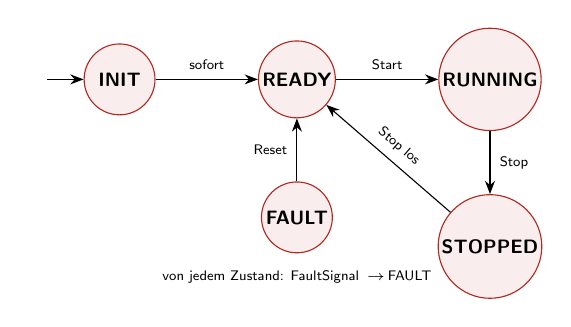
\begin{tikzpicture}[>=Stealth, node distance=8mm and 13mm,
  every state/.style={minimum size=9mm, inner sep=1pt, font=\scriptsize\bfseries,
    draw=cB5, fill=cB5!8}, every edge/.style={draw, ->}, font=\tiny]
\node[state, initial, initial text=] (I) {INIT};
\node[state, right=of I] (R) {READY};
\node[state, right=of R] (U) {RUNNING};
\node[state, below=of U] (S) {STOPPED};
\node[state, below=of R] (F) {FAULT};
\path (I) edge node[above] {sofort} (R)
      (R) edge node[above] {Start} (U)
      (U) edge node[right] {Stop} (S)
      (S) edge node[above, sloped] {Stop los} (R)
      (F) edge node[left] {Reset} (R);
\node[font=\tiny, below=1mm of F] {von jedem Zustand: FaultSignal \ra FAULT};
\end{tikzpicture}
\end{center}
\begin{lstlisting}
TYPE EN_FOERDERBAND_ZUSTAND :
  (INIT, READY, RUNNING, STOPPED, FAULT);
END_TYPE

FUNCTION_BLOCK FB_FOERDERBAND_LOGIK
VAR_INPUT
  StartButton, StopButton, FaultSignal, ResetButton : BOOL;
END_VAR
VAR_OUTPUT ConveyorOn, FaultIndicator : BOOL; END_VAR
VAR
  eZustand : EN_FOERDERBAND_ZUSTAND := INIT;
  rtStart, rtReset : R_TRIG;
END_VAR

rtStart(CLK := StartButton);
rtReset(CLK := ResetButton);
IF FaultSignal THEN eZustand := FAULT; END_IF  // gilt überall

CASE eZustand OF
  INIT:    eZustand := READY;
  READY:   IF rtStart.Q THEN eZustand := RUNNING; END_IF
  RUNNING: IF StopButton THEN eZustand := STOPPED; END_IF
  STOPPED: IF NOT StopButton THEN eZustand := READY; END_IF
  FAULT:   IF rtReset.Q AND NOT FaultSignal THEN
             eZustand := READY;
           END_IF
END_CASE

ConveyorOn     := (eZustand = RUNNING);
FaultIndicator := (eZustand = FAULT);
\end{lstlisting}
\begin{lstlisting}
PROGRAM MAIN
VAR
  bStart  AT %I* : BOOL;   bStop  AT %I* : BOOL;
  bFault  AT %I* : BOOL;   bReset AT %I* : BOOL;
  bMotor  AT %Q* : BOOL;   bLampe AT %Q* : BOOL;
  fbBand1 : FB_FOERDERBAND_LOGIK;
END_VAR
fbBand1(StartButton := bStart, StopButton := bStop,
        FaultSignal := bFault, ResetButton := bReset,
        ConveyorOn => bMotor, FaultIndicator => bLampe);
\end{lstlisting}
\begin{formel}[(e) Zweites Förderband]
\label{falle:instanz}
Zweite \T{Instanz} \R{fbBand2 : FB\_FOERDERBAND\_LOGIK;} plus eigene
E/A-Variablen (\R{AT \%I*}/\R{AT \%Q*}) deklarieren, verknüpfen und
\R{fbBand2(...)} aufrufen. Der FB-Code bleibt unverändert -- jede Instanz
hat ihren eigenen \R{eZustand}. Genau darum gehört die Logik in einen FB
und nicht ins Programm.
\end{formel}

\subsection{MEP HS24: Ampel für eine Kreuzung}
\label{bsp:ampel}
\begin{lstlisting}
TYPE EN_FARBEN        : (ROT, GELB, GRUEN);      END_TYPE
TYPE EN_BETRIEBSMODUS : (AUTOMATIK, MANUELL);    END_TYPE
TYPE EN_PHASE : (A_GRUEN, A_GELB, B_GRUEN, B_GELB); END_TYPE

VAR_GLOBAL   // GVL_IO
  bA_Rot AT %Q* : BOOL; bA_Gelb AT %Q* : BOOL; bA_Gruen AT %Q* : BOOL;
  bB_Rot AT %Q* : BOOL; bB_Gelb AT %Q* : BOOL; bB_Gruen AT %Q* : BOOL;
  bTA_Rot AT %I* : BOOL; bTA_Gelb AT %I* : BOOL; bTA_Gruen AT %I* : BOOL;
  bTB_Rot AT %I* : BOOL; bTB_Gelb AT %I* : BOOL; bTB_Gruen AT %I* : BOOL;
  bHand   AT %I* : BOOL;              // Wahlschalter Handbetrieb
END_VAR

PROGRAM MAIN
VAR
  eModus  : EN_BETRIEBSMODUS := AUTOMATIK;
  arAmpel : ARRAY[1..2] OF EN_FARBEN := [ROT, ROT];
  ePhase  : EN_PHASE := A_GRUEN;
  tonGruen, tonGelb : TON;
END_VAR

IF GVL_IO.bHand THEN eModus := MANUELL; ELSE eModus := AUTOMATIK; END_IF

CASE eModus OF
AUTOMATIK:
  tonGruen(IN := (ePhase = A_GRUEN) OR (ePhase = B_GRUEN), PT := T#10S);
  tonGelb (IN := (ePhase = A_GELB)  OR (ePhase = B_GELB),  PT := T#3S);
  CASE ePhase OF
    A_GRUEN: arAmpel[1] := GRUEN; arAmpel[2] := ROT;
             IF tonGruen.Q THEN ePhase := A_GELB; END_IF
    A_GELB:  arAmpel[1] := GELB;  arAmpel[2] := ROT;
             IF tonGelb.Q THEN ePhase := B_GRUEN; END_IF
    B_GRUEN: arAmpel[1] := ROT;   arAmpel[2] := GRUEN;
             IF tonGruen.Q THEN ePhase := B_GELB; END_IF
    B_GELB:  arAmpel[1] := ROT;   arAmpel[2] := GELB;
             IF tonGelb.Q THEN ePhase := A_GRUEN; END_IF
  END_CASE
MANUELL:   // Grün nur, wenn die andere Ampel nicht grün ist
  IF GVL_IO.bTA_Rot THEN arAmpel[1] := ROT;
  ELSIF GVL_IO.bTA_Gelb THEN arAmpel[1] := GELB;
  ELSIF GVL_IO.bTA_Gruen AND arAmpel[2] <> GRUEN THEN arAmpel[1] := GRUEN;
  END_IF
  IF GVL_IO.bTB_Rot THEN arAmpel[2] := ROT;
  ELSIF GVL_IO.bTB_Gelb THEN arAmpel[2] := GELB;
  ELSIF GVL_IO.bTB_Gruen AND arAmpel[1] <> GRUEN THEN arAmpel[2] := GRUEN;
  END_IF
END_CASE

GVL_IO.bA_Rot := arAmpel[1] = ROT;  GVL_IO.bA_Gelb := arAmpel[1] = GELB;
GVL_IO.bA_Gruen := arAmpel[1] = GRUEN;
GVL_IO.bB_Rot := arAmpel[2] = ROT;  GVL_IO.bB_Gelb := arAmpel[2] = GELB;
GVL_IO.bB_Gruen := arAmpel[2] = GRUEN;
\end{lstlisting}
\begin{falle}[Ampel: was man begründen sollte]
Zwei Timer reichen, weil zwischen zwei Grünphasen immer eine Gelbphase
liegt (\R{IN} fällt dazwischen ab \ra Reset). Rot einer Ampel dauert hier
Grün $+$ Gelb der anderen $=13$\,s; exakt 10\,s Rot ginge nur mit
kürzerer Grünphase der Gegenrichtung. „Nie beide grün“ ist in Automatik
durch die Phasen garantiert, im Handbetrieb durch die Verriegelung.
\end{falle}

\subsection{Weitere Automaten aus AS 4}
\SW{Safe} Init (Code-Array füllen) \ra Close (Zähler/Lampen reset) \ra
CheckDigit (nur bei \R{risingEdge}, 4 Tasten, \R{correctCounter},
\R{currentIndex}) \ra Open (grün, \R{lightDuration} 5\,s) bzw.\ WrongCode
(rot, 5\,s) \ra Close. Zusatz: Doppelklick blau bricht ab; Code im Zustand
Open mit beiden Tasten neu programmieren.
\SW{Ampel-FB} Eingänge \R{clear\_road}, \R{block\_road},
\R{disable\_system}; Init \ra Red \ra(clear) Red\&Yellow \ra(2\,s) Green
\ra(block) Yellow \ra(5\,s) Red; Disabled: gelb blinkt 1\,s, zurück zu Red,
wenn \R{disable} weg. Als FB \ra Kreuzung $=$ 4 Instanzen, Phase A
(Ampel 1+3, 5\,s), Phase B (2+4, 8\,s), dazwischen sicherer Wechsel.

  % !TEX root = ../main.tex
% ---------------------------------------------------------------------
%  B6 -- Tasks, Echtzeit, EtherCAT (Skript Kap. 7; AS 6)
% ---------------------------------------------------------------------
\vlsec{cB6}{B6}{Tasks, Echtzeit, EtherCAT}
\label{sec:tasks}

\SW{Task} Ausführungseinheit: ruft die zugeordneten Programme mit fester
\T{Zykluszeit} und \T{Priorität} auf. Mehrere Tasks \ra verschiedene
Programme mit verschiedenen Zykluszeiten im selben Projekt.
\SW{Determinismus} Programm läuft exakt alle $T$. Schwankung $=$
\T{Jitter} \ra Regler stimmt nicht mehr (Entwurf setzt konstantes $T$
voraus), Roboter positioniert falsch, Druck an falscher Stelle.

\begin{formel}[Prioritäten in TwinCAT]
\T{Präemptiv}: Wird ein höher priorer Task fällig, wird der laufende
niedriger priore unterbrochen und später fortgesetzt.\\
\T{1 $=$ höchste} Priorität. \T{Jede Prioritätsstufe nur für genau einen
Task} -- zwei Tasks mit gleicher Priorität geht nicht.\\
Zykluszeit $=$ ganzzahliges Vielfaches der \T{Basiszeit} (SYSTEM \ra
Echtzeit), eingestellt in Zyklusticks.
\end{formel}
\begin{falle}[Zykluszeit und CPU-Last]
Kürzere Zykluszeit \ra Programm läuft öfter \ra \emph{höhere}
CPU-Auslastung. Last je Task $=\frac{\text{Laufzeit}}{\text{Zykluszeit}}$.
Summe $>100\,\%$ \ra Überlast, niedrig priore Tasks verpassen ihren Zyklus.
\end{falle}

\begin{bsp}[AS 6: drei Tasks, je 30\,$\mu$s Rechenzeit]
\label{bsp:tasks}
FastTask 300\,$\mu$s Prio 2, Standard 1\,ms Prio 1, SlowTask 10\,ms Prio 3.\\
\T{Basiszeit}: muss 300\,$\mu$s und 1\,ms teilen \ra $\text{ggT}=100\,\mu$s.\\
\T{Last}: $\frac{30}{300}+\frac{30}{1000}+\frac{30}{10000}=10+3+0.3=13.3\,\%$.\\
\T{$t=0$} (alle fällig): Standard 0--30, Fast 30--60, Slow 60--90\,$\mu$s.\\
\T{$t=3$\,ms} (Fast + Standard): Standard zuerst, Fast 30\,$\mu$s zu spät
\ra Jitter für Fast. Sonst laufen die Tasks allein.\\
\T{Lehre:} Der schnellste Task sollte die höchste Priorität haben, sonst
wird gerade er verzögert.
\end{bsp}

\subsection{EtherCAT}
\label{sec:ethercat}
\begin{formel}[Funktionsprinzip]
Normales Ethernet-Frame, \T{Ethertype \R{0x88A4}}. Der Master (SPS)
sendet ein Frame mit allen Ausgangsdaten; es läuft \emph{seriell} durch alle
Klemmen, die letzte schickt es zurück (Ring). Jede Klemme entnimmt ihre
Ausgänge und setzt ihre Eingänge ein.\\
\T{On-the-fly}: Verarbeitung \emph{während} das Frame durchläuft
(ns Verzögerung) statt empfangen-verarbeiten-senden.\\
\T{In-place}: Eingangsdaten überschreiben bereits gelesene Ausgangsdaten
\ra Frame bleibt kurz.\\
Master-Netzwerkkarte schreibt per \T{DMA} direkt ins RAM \ra
Protokollbearbeitung in Hardware, unabhängig von CPU-Last.
\end{formel}
\SW{Zahlen} Zyklen $\le100\,\mu$s; 256 verteilte DIO in 10\,$\mu$s,
1000 DIO in 30\,$\mu$s; Synchronisation (Distributed Clocks) Jitter
$\le1\,\mu$s; offener Standard (ETG), günstige Standard-Hardware.
\SW{Frames} Pro Task mit E/A ein eigenes Frame/Zyklus (Reiter EtherCAT
am Gerät, Spalte Cycle).
\SW{EL6601} Standard-Ethernet in den Lücken zwischen EtherCAT-Frames.
\SW{XFC / Oversampling} z.\,B.\ EL1262: $n$ Abtastungen pro Buszyklus
($1\,\text{ms}/n=10$ \ra 100\,$\mu$s), gesammelt übertragen.

\begin{ztab}{@{}lX@{}}
Begriff & Bedeutung \\ \midrule
Working Counter (WC) & Jede Klemme, die ihr Datagramm bearbeitet,
  erhöht den WC. Master vergleicht mit Sollwert: Abweichung \ra Daten
  dieser Gruppe ungültig, Diagnose. \\
Sync Unit & Gruppe von Klemmen mit eigenem WC. Fällt eine Gruppe aus,
  bleiben die Daten der anderen gültig. Konfiguration am EtherCAT-Gerät
  (Sync-Unit-Zuordnung). \\
Hot Connect & Gerätegruppen, die im Betrieb an- und abgesteckt werden
  dürfen (Werkzeugwechsler, modulare Maschinenteile) -- typischer Fall,
  wo Sync Units unabdingbar sind. \\
\end{ztab}

  % !TEX root = ../main.tex
% ---------------------------------------------------------------------
%  B7 -- PID-Regler und Anti-Reset-Windup (Skript Kap. 8/9; AS 7/8;
%        Folien Reglerdiskretisierung; Skript Digitale Regelung Kap. 4)
% ---------------------------------------------------------------------
\vlsec{cB7}{B7}{PID-Regler und Anti-Reset-Windup}
\label{sec:pid}

\SW{Regelkreis} Sollwert $r$, Regelgrösse $y$, Regeldifferenz
$e=r-y$, Steuergrösse $u$, Störgrösse; Regler $C(s)$, Strecke $G(s)$.
Digital: AD-Wandlung \ra $e(k)$ \ra Regelalgorithmus \ra DA-Wandlung, alle
$T$ einmal.
\begin{ztab}{@{}lX@{}}
Anteil & Wirkung \\ \midrule
P ($K_p$) & sofort proportional; bleibender Fehler (ausser integrierende
  Strecke); zu gross \ra instabil \\
I ($T_i$) & summiert $e$ \ra kein bleibender Fehler; träge,
  Überschwingen, Windup \\
D ($T_d$) & reagiert auf Änderungsrate, dämpft; verstärkt Rauschen \ra
  immer mit Tiefpass ($N$) \\
\end{ztab}
\begin{formel}[Realer PID (Labor-Form)]
\[C(s)=\frac{U(s)}{E(s)}=K_p\Big(1+\frac{1}{T_is}+\frac{T_ds}{\frac{T_d}{N}s+1}\Big)\]
$T_i$ Nachstellzeit, $T_d$ Vorhaltzeit, $T_d/N$ Filterzeitkonstante
($N\approx1..100$, Labor 20). Umrechnung: $K_i=K_p/T_i$, $K_d=K_pT_d$.\\
\T{D auf $y$ statt $e$}: Sollwertsprünge würden einen Stoss erzeugen
\ra $u_d$ aus $-y$ berechnen (Minuszeichen!).
\end{formel}
\SW{Indirekter Entwurf} (Labor): analog entwerfen, dann diskretisieren
\ra keine neuen Methoden, intuitiv; aber nur PID und Abtastung nicht
explizit berücksichtigt. \T{Direkt}: Strecke $H(z)$, digital entwerfen.

\subsection{Diskretisierung der drei Anteile}
\label{rez:pid}
\begin{ztab}{@{}lX@{}}
P & $u_p(k)=K_p\,e(k)$ \\
I Rechteck rückw. & $u_i(k)=u_i(k-1)+\frac{K_pT}{T_i}\,e(k)$ \\
I Rechteck vorw. & $u_i(k)=u_i(k-1)+\frac{K_pT}{T_i}\,e(k-1)$ \\
\T{I Trapez} & $u_i(k)=u_i(k-1)+\frac{K_pT}{2T_i}\big(e(k)+e(k-1)\big)$ \\
D ungefiltert & $u_d(k)=\frac{K_pT_d}{T}\big(e(k)-e(k-1)\big)$ \\
\T{D gefiltert} & $u_d(k)=\frac{T_d}{T_d+NT}\,u_d(k-1)+\frac{K_pT_dN}{T_d+NT}\big(e(k)-e(k-1)\big)$ \\
D auf $y$ & wie oben mit $-\big(y(k)-y(k-1)\big)$ statt $\Delta e$ \\
Summe & $u(k)=u_p(k)+u_i(k)+u_d(k)$ \\
\end{ztab}
\begin{formel}[Herleitung D gefiltert (Rückwärts-Rechteck)]
$\big(\tfrac{T_d}{N}s+1\big)U_d=K_pT_d\,s\,E$, mit $s\to\frac{1-z^{-1}}{T}$:
\[\frac{T_d}{NT}\big(u_d(k)-u_d(k-1)\big)+u_d(k)=\frac{K_pT_d}{T}\big(e(k)-e(k-1)\big)\]
Mal $NT$: $(T_d+NT)\,u_d(k)=T_d\,u_d(k-1)+K_pT_dN\,\Delta e$
\ra nach $u_d(k)$ auflösen \ra Tabelle.\\
Summe \ra Rekursion: $\sum_{i=0}^{k}=\sum_{i=0}^{k-1}+$ neuer Summand
\ra konstante Rechenzeit und Speicher.
\end{formel}

\subsection{Virtuelle Strecke PT1T2 (AS 7)}
$G(s)=\frac{K}{(1+T_1s)(1+T_2s)}$, $a_1=e^{-T/T_1}$, $a_2=e^{-T/T_2}$:
\[H(z)=\frac{b_0z+b_1}{z^2+c_1z+c_2},\quad c_1=-(a_1+a_2),\; c_2=a_1a_2\]
\[b_0=\tfrac{K}{T_1-T_2}\big[T_1(1-a_1)-T_2(1-a_2)\big]\]
\[b_1=\tfrac{K}{T_1-T_2}\big[T_2a_1(1-a_2)-T_1a_2(1-a_1)\big]\]
\[y(k)=-c_1y(k-1)-c_2y(k-2)+b_0u(k-1)+b_1u(k-2)\]
\SW{Test} $K=10$, $T_1=0.1$, $T_2=0.01$; Regler $K_p=1/K$, $T_i=T_1$,
$T_d=T_2$ (kürzt die Strecken-Pole).

\subsection{Init/Run-Muster}
\label{sec:initrun}
Konstante Koeffizienten nur \emph{einmal} im Init rechnen, im Run nur die
Differenzengleichung \ra minimale CPU-Last pro Zyklus.
\begin{lstlisting}
TYPE System_Modus_Enum : (System_Init, System_Run); END_TYPE
TYPE PID_Parameter_Strukt :
STRUCT
  Kp, Ti, Td : REAL;  N : UINT;   ARW : BOOL;
  umin, umax, Tr : REAL;
END_STRUCT
END_TYPE

FUNCTION_BLOCK PID_Regler
VAR_INPUT
  r, y : REAL;  Modus : System_Modus_Enum;
  Param : PID_Parameter_Strukt;  T : REAL;
END_VAR
VAR_OUTPUT u, usat : REAL; END_VAR
VAR
  e, e1, y1, up, ui, ud : REAL;
  ci, cd1, cd2 : REAL;               // vorberechnete Koeffizienten
END_VAR

CASE Modus OF
System_Init:
  ci  := Param.Kp * T / (2.0 * Param.Ti);
  cd1 := Param.Td / (Param.Td + UINT_TO_REAL(Param.N) * T);
  cd2 := Param.Kp * Param.Td * UINT_TO_REAL(Param.N)
         / (Param.Td + UINT_TO_REAL(Param.N) * T);
  ui := 0.0; ud := 0.0; e1 := 0.0; y1 := y;
System_Run:
  e  := r - y;
  up := Param.Kp * e;
  ud := cd1 * ud - cd2 * (y - y1);         // D auf y
  u  := up + ui + ud;                      // ui(k-1)!
  IF u > Param.umax THEN usat := Param.umax;    // Sättigung
  ELSIF u < Param.umin THEN usat := Param.umin;
  ELSE usat := u; END_IF
  ui := ui + ci * (e + e1);                // Trapez
  IF Param.ARW THEN                        // Back-Calculation
    ui := ui + T / Param.Tr * (usat - u);
  END_IF
  e1 := e;  y1 := y;
END_CASE
\end{lstlisting}

\subsection{Stellgrössenbegrenzung und Anti-Reset-Windup}
\label{sec:arw}
\SW{Sättigung} Jeder Aktor ist begrenzt (Ventil offen, Spannung):
$u_{\text{sat}}=u_{\max}$ wenn $u\ge u_{\max}$, $u_{\min}$ wenn
$u\le u_{\min}$, sonst $u$. Die Begrenzung gehört physikalisch zur
Strecke, der Regler muss $u_{\text{sat}}$ aber kennen.
\begin{formel}[Windup]
Ist $u$ lange am Anschlag, integriert der I-Anteil die Regeldifferenz
ungebremst weiter, obwohl mehr Stellgrösse nicht wirkt. Nach dem
Vorzeichenwechsel von $e$ muss er erst wieder abgebaut werden \ra starkes,
langes \T{Überschwingen}, träge Reaktion auf neuen Sollwert, eventuell
Zahlenüberlauf.
\end{formel}
\begin{ztab}{@{}lX@{}}
Massnahme & Prinzip \\ \midrule
Conditional Integration & I-Anteil anhalten, solange gesättigt (und $e$
  weiter in dieselbe Richtung zeigt). Einfach, dynamisch nicht optimal. \\
\T{Back-Calculation} & Differenz $u_{\text{sat}}-u$ mit $\frac{1}{T_r}$
  gewichtet vor den Integrator zurückführen. Ohne Sättigung ist die
  Differenz 0 \ra kein Einfluss. \\
\end{ztab}
\begin{formel}[ARW diskret (Folien)]
$u_{\text{nosat}}(k)=u_p(k)+u_i(k-1)+u_d(k)$ \ra begrenzen \ra
\[u_i(k)=u_i(k-1)+\frac{K_pT}{T_i}\,\frac{e(k)+e(k-1)}{2}
+\frac{T}{T_r}\big(u_{\text{sat}}(k)-u_{\text{nosat}}(k)\big)\]
Startwert $T_r=\sqrt{T_iT_d}$ oder $\frac{T_i+T_d}{2}$ (Labor
Motor: $T_r=\sqrt{T_iT_d}$, $N=20$).
\end{formel}
\SW{Test AS 8} $u_{\min}=0$, $u_{\max}=10$; Sollwert als PWM 25 \ra 75;
$K_p\in\{\frac1K,\frac{10}{K},\frac{100}{K}\}$ -- hohe Verstärkung zeigt
den Windup am deutlichsten; wird es instabil, $T$ verkleinern.

\subsection{Laborversuch (Semesterleistung)}
SPS: Messsignale im Scope, Aktoren im Config-Modus, Zustandsmaschine
Hand/Auto bzw.\ Open-/Closed-Loop in \R{MAIN}, PID-FB, Prozess-FB.
Identifikation per \T{Sprungantwort} ($K,\tau_1,\tau_2$), Entwurf
(Ziegler-Nichols, SISO-Tool), Reserven: Phase $\ge50^\circ$,
Amplitude $\ge8$\,dB. Encoder EL5101 zählt alle Flanken von A und B
\ra $4\times$ Auflösung (512 \ra 2048/Umdrehung); Zählerüberlauf abfangen.
Motor EL7342: $\pm32767\leftrightarrow\pm24$\,V.

  % !TEX root = ../main.tex
% ---------------------------------------------------------------------
%  B8 -- Funktionale Sicherheit, TwinSAFE (Skript Kap. 10; AS 9)
% ---------------------------------------------------------------------
\vlsec{cB8}{B8}{Funktionale Sicherheit und TwinSAFE}
\label{sec:safety}

\SW{Funktionale Sicherheit} Die Steuerung schützt Personen und Umwelt,
nicht nur den Betrieb. Oft sicherer, kontrolliert zu stoppen als einfach
die Energie zu kappen \ra Not-Halt, Schutztür, Zweihand in die SPS.
\begin{ztab}{@{}lX@{}}
Norm & Einstufung \\ \midrule
IEC 61508 & E/E/PE-Systeme allgemein: \T{SIL 1--4} (4 $=$ höchste) \\
ISO 13849-1 & Maschinen: \T{PL a--e}, Kategorien B, 1--4 \\
\end{ztab}
\begin{formel}[Grundprinzip]
\T{Redundanz} (1oo2): zwei Kanäle/Controller rechnen und vergleichen
sich gegenseitig. Abweichung \ra \T{Fail-Safe}: sicherer Zustand
(abschalten statt fehlerhaft weiterlaufen).
\T{Diagnosedeckungsgrad}: wie viele Fehler erkannt werden.
\T{Common Cause Failure}: eine Ursache (Überspannung) darf nicht beide
Kanäle gleichzeitig ausschalten \ra getrennte Versorgung.
\end{formel}

\subsection{TwinSAFE-Klemmen}
\begin{ztab}{@{}lX@{}}
EL6900 & TwinSAFE-Logic: „zweite SPS“ für Safety, Programm läuft auf
  \emph{zwei} Controllern, Ergebnisse verglichen; bis 128 Verbindungen;
  SIL 3 / PL e \\
EL1904 & 4 sichere Eingänge, zwei Controller mit eigener Versorgung,
  Testpulse erkennen Drahtbruch (nur mit NC-Kontakten, \emph{Sensortest
  active}) \\
EL2904 & 4 sichere Ausgänge, 24\,V, 0.5\,A je Kanal, doppelt ausgeführt \\
\end{ztab}
Gelb markiert, Bezeichnung \R{x9xx}. Sicherheitsprotokoll eingebettet im
normalen EtherCAT-Telegramm \ra gleicher Bus wie Standard-Klemmen.

\begin{rezept}[Safety-Projekt (AS 9)]
\begin{enumerate}
\item E/A scannen: EL6900, EL1904, EL2904 sichtbar.
\item SAFETY \ra neues TwinSAFE-Projekt, Target \emph{Hardware Safety
  PLC}, Physical Device $=$ EL6900.
\item TwinSAFE-Gruppe, Alias Devices EL1904/EL2904 hinzufügen und mit
  der Klemme verbinden.
\item Logik in der \R{.sal}-Datei \T{grafisch} aus validierten
  \R{safe}-Bausteinen (nicht ST); Ein-/Ausgänge benennen, im Variable
  Mapping verknüpfen.
\end{enumerate}
\end{rezept}
\begin{falle}[Not-Aus \ra Relais]
Normalzustand: Not-Aus nicht gedrückt, Relais \emph{an}. Ruhestromprinzip:
Drahtbruch oder Stromausfall muss wie „Not-Aus gedrückt“ wirken
(NC-Kontakt, Testpulse) \ra Relais \emph{aus}. Nach dem Lösen nicht
automatisch wieder anlaufen: Quittierung (Reset-Taster) verlangen.
\end{falle}

  % !TEX root = ../main.tex
% ---------------------------------------------------------------------
%  Referenz: Fragebogen, Formeln, Prüfungs-Checkliste
% ---------------------------------------------------------------------
\vlsec{cREF}{REF}{Prüfungsreferenz}
\label{sec:referenz}

\subsection{Fragebogen MEP HS24 mit Begründung}
\label{sec:quiz}
\begin{ztab}{@{}rXl@{}}
\# & Aussage \ra Begründung & \\ \midrule
1 & ST + \emph{fünf weitere} Sprachen \ra es sind 5 insgesamt (ST + 4) & \NEIN \\
2 & IEC 61131-3 nur von Beckhoff \ra herstellerübergreifende Norm & \NEIN \\
3 & Zuerst Ausgänge setzen, dann Eingänge lesen \ra umgekehrt (PAE, Programm, PAA) & \NEIN \\
4 & 200\,$\mu$s Abtastzeit mit TwinCAT/EtherCAT \ra EtherCAT $\le100\,\mu$s, Tasks 300\,$\mu$s im Labor & \JA \\
5 & TwinCAT-Programm wird immer zyklisch aufgerufen \ra jedes PROGRAM hängt an einem Task & \JA \\
6 & EtherCAT ist TCP/IP-basiert \ra eigener Ethertype auf Schicht 2 & \NEIN \\
7 & FB mit Gedächtnis muss nicht instanziiert werden \ra muss & \NEIN \\
8 & GVL nur für Klemmen-Variablen \ra auch Konstanten, globale Daten & \NEIN \\
9 & ENUM beginnt immer bei 0 \ra Werte frei setzbar (\R{JANUAR:=1}) & \NEIN \\
10 & Zykluszeit mehrere Sekunden möglich \ra Vielfaches der Basiszeit; \emph{nicht im Skript bestätigt} & (Ja?) \\
11 & Verschiedene Zykluszeiten für verschiedene Programme \ra mehrere Tasks & \JA \\
12 & TwinCAT ist ein Feldbus \ra Software; Feldbus ist EtherCAT & \NEIN \\
13 & Zykluszeit ohne Einfluss auf CPU-Last \ra kürzer $=$ mehr Last & \NEIN \\
14 & Mehrere INT aus FB nur via Struktur/Array \ra mehrere \R{VAR\_OUTPUT} & \NEIN \\
15 & Mehrere Tasks mit gleicher Priorität \ra jede Stufe nur ein Task & \NEIN \\
16 & FUNCTION speichert Inhalt zwischen Aufrufen \ra kein Gedächtnis & \NEIN \\
\end{ztab}
\begin{falle}[Wertung]
$+1$ richtig, $-1$ falsch, 0 leer. Frage 10 ist nicht durch die
Unterlagen belegt \ra im Zweifel leer lassen.
\end{falle}

\subsection{Alle Formeln auf einen Blick}
\begin{ztab}{@{}lX@{}}
Analog-Eingang & $U=\frac{\text{INT}}{32767}\cdot10$\,V \\
Analog-Ausgang & $\text{INT}=\text{REAL\_TO\_INT}(U/10\cdot32767)$ \\
Lineare Kennlinie & $p=p_1+(U-U_1)\frac{p_2-p_1}{U_2-U_1}$ \\
Blinken mit $f$ & Timer-\R{PT} $=\frac{1}{2f}$ (3\,Hz \ra 167\,ms) \\
PWM & $N_2=T_0/T$, $N_1=\text{Duty}\cdot N_2$ \\
Mittelwert rekursiv & $M(k)=M(k-1)+\frac1N(y(k)-y(k-N-1))$ \\
Forgetting Factor & $M(k)=\lambda M(k-1)+(1-\lambda)y(k)$ \\
Euler rückwärts & $s=\frac{1-z^{-1}}{T}$ \\
Tustin & $s=\frac2T\frac{1-z^{-1}}{1+z^{-1}}$ \\
PT1 diskret & $y(k)=\frac{\tau}{\tau+T}y(k-1)+\frac{T}{\tau+T}u(k)$ \\
I Trapez & $u_i(k)=u_i(k-1)+\frac{K_pT}{2T_i}(e(k)+e(k-1))$ \\
D gefiltert & $u_d(k)=\frac{T_d}{T_d+NT}u_d(k-1)+\frac{K_pT_dN}{T_d+NT}\Delta e$ \\
ARW & $+\frac{T}{T_r}(u_{\text{sat}}-u)$ im I-Anteil, $T_r=\sqrt{T_iT_d}$ \\
Stabilität diskret & alle Pole $|p|<1$ \\
Abtasttheorem & $\omega_s>2\omega_{\max}$; $T\le0.1\,T_1$ \\
Task-Last & $\sum\frac{\text{Laufzeit}}{\text{Zykluszeit}}$; Basiszeit $=$ ggT \\
Shift & \R{SHR(x,n)} $=x/2^n$, \R{SHL(x,n)} $=x\cdot2^n$ \\
\end{ztab}

\subsection{Code auf Papier -- Checkliste}
\begin{rezept}[Bevor du abgibst]
\begin{enumerate}
\item Jede Variable deklariert? E/A mit \R{AT \%I*}/\R{AT \%Q*},
  in GVL mit \R{GVL\_IO.}-Präfix verwendet?
\item Typen passen? \R{INT\_TO\_REAL} vor dem Rechnen, \R{10.0} statt
  \R{10}, Rückgabetyp der Funktion gesetzt.
\item FB \emph{instanziiert} und \emph{jeden Zyklus} aufgerufen? Timer
  und Flanken ausserhalb von \R{IF}/\R{CASE}-Zweigen.
\item Taster in Transitionen über Flanke (\R{R\_TRIG}/EdgeDetector).
\item Speicher nachgeschoben ($y_2:=y_1$, dann $y_1:=y$)?
\item Division durch 0 abgefangen, \R{WHILE} vermieden.
\item Jedes \R{IF} mit \R{END\_IF}, \R{CASE} mit \R{END\_CASE}, Semikolons.
\item Kurz kommentieren, \emph{warum} (z.\,B.\ „FUNCTION reicht, kein
  Gedächtnis“) -- Begründungen geben Punkte.
\end{enumerate}
\end{rezept}

  % !TEX root = ../main.tex
% ---------------------------------------------------------------------
%  Stichwortregister -- vom Begriff zur Abschnittsnummer
%  ERZEUGT von mkreg.py. Neue Eintraege dort ergaenzen und neu laufen
%  lassen, oder hier von Hand alphabetisch einsortieren.
% ---------------------------------------------------------------------
\vlsec{cREF}{REF}{Stichwortregister}

\scriptsize
\begin{tabularx}{\linewidth}{@{}Xr@{\hskip6pt}Xr@{}}
Abtasttheorem & \ref{rez:diskret} & Init/Run & \ref{sec:initrun} \\
ADS / AMS Net Id & \ref{sec:twincat} & Instanz & \ref{falle:instanz} \\
Aliasing & \ref{rez:diskret} & ISO 13849 / PL & \ref{sec:safety} \\
Ampel (MEP) & \ref{bsp:ampel} & Ja/Nein-Fragen & \ref{sec:quiz} \\
Anti-Reset-Windup & \ref{sec:arw} & Jitter & \ref{sec:tasks} \\
\R{AT \%I*} / \R{\%Q*} & \ref{rez:gvlio} & Mittelwert gleitend & \ref{sec:mittelwert} \\
Automatisierungspyramide & \ref{sec:grundlagen} & NOVRAM / USV & \ref{sec:remanenz} \\
Back-Calculation & \ref{sec:arw} & On-the-fly / in-place & \ref{sec:ethercat} \\
Basiszeit & \ref{bsp:tasks} & PAE / PAA & \ref{sec:twincat} \\
Bibliothek & \ref{sec:biblio} & PERSISTENT & \ref{sec:remanenz} \\
Butterworth & \ref{bsp:fbfilter} & PID-Regler & \ref{sec:pid} \\
\R{CASE} & \ref{rez:automat} & PLCopenXML & \ref{sec:biblio} \\
CoE / CoE-Startup & \ref{sec:twincat} & Priorität & \ref{sec:tasks} \\
Conditional Integration & \ref{sec:arw} & PT1 / PT2 & \ref{rez:diskret} \\
D-Anteil gefiltert & \ref{rez:pid} & PT1T2-Strecke & \ref{sec:initrun} \\
Differenzengleichung & \ref{rez:diskret} & PWM & \ref{sec:signale} \\
Doppelklick & \ref{bsp:edge} & Redundanz 1oo2 & \ref{sec:safety} \\
DUT & \ref{sec:st} & RETAIN & \ref{sec:remanenz} \\
EdgeDetector & \ref{bsp:edge} & Route & \ref{sec:twincat} \\
EL3004 & \ref{sec:twincat} & \R{R\_TRIG} & \ref{sec:timer} \\
EL6900 / EL1904 / EL2904 & \ref{sec:safety} & Scan-Zyklus & \ref{sec:twincat} \\
EN 61499 & \ref{sec:sprachen} & Schaltschrank & \ref{sec:grundlagen} \\
ENUM & \ref{sec:st} & Sensor skalieren & \ref{rez:skalierung} \\
EtherCAT & \ref{sec:ethercat} & \R{SHL} / \R{SHR} & \ref{rez:statuswort} \\
Euler vorw./rückw. & \ref{rez:diskret} & Statuswort & \ref{rez:statuswort} \\
\R{EXIT} & \ref{sec:st} & Steuern vs. Regeln & \ref{sec:grundlagen} \\
Fail-Safe & \ref{sec:safety} & STRUCT & \ref{sec:st} \\
Feldbus & \ref{sec:feldbus} & Sync Unit & \ref{sec:ethercat} \\
FIR / IIR & \ref{rez:diskret} & Task & \ref{sec:tasks} \\
Flanke & \ref{bsp:edge} & \R{TON} / \R{TOF} / \R{TP} & \ref{sec:timer} \\
Förderband (MEP) & \ref{bsp:foerderband} & Tustin & \ref{rez:diskret} \\
Forgetting Factor & \ref{sec:mittelwert} & Typkonvertierung & \ref{sec:st} \\
Freerun / Config & \ref{sec:twincat} & UML-Statechart & \ref{sec:automaten} \\
Funktion / FB / Programm & \ref{sec:pou} & \R{WHILE}-Falle & \ref{sec:st} \\
GVL & \ref{rez:gvlio} & Working Counter & \ref{sec:ethercat} \\
Hot Connect & \ref{sec:ethercat} & z-Transformation & \ref{rez:diskret} \\
I-Anteil Trapez & \ref{rez:pid} & Zustandsautomat & \ref{rez:automat} \\
IEC 61131-3 & \ref{sec:sprachen} & Zweierkomplement & \ref{sec:st} \\
IEC 61508 / SIL & \ref{sec:safety} &  &  \\
\end{tabularx}
\normalsize

\end{multicols*}

\end{document}
